\def\year{2020}\relax
%File: formatting-instruction.tex
\documentclass[letterpaper, twocolumn]{article} % DO NOT CHANGE THIS
% \usepackage{aaai20}  % DO NOT CHANGE THIS
\usepackage[left=1in,right=1in]{geometry}

\usepackage{times}  % DO NOT CHANGE THIS
\usepackage{helvet} % DO NOT CHANGE THIS
\usepackage{courier}  % DO NOT CHANGE THIS
\usepackage[hyphens]{url}  % DO NOT CHANGE THIS
\usepackage{graphicx} % DO NOT CHANGE THIS
\urlstyle{rm} % DO NOT CHANGE THIS
\def\UrlFont{\rm}  % DO NOT CHANGE THIS
\usepackage{graphicx}  % DO NOT CHANGE THIS
\frenchspacing  % DO NOT CHANGE THIS
\setlength{\pdfpagewidth}{8.5in}  % DO NOT CHANGE THIS
\setlength{\pdfpageheight}{11in}  % DO NOT CHANGE THIS
%\nocopyright
%PDF Info Is REQUIRED.
% For /Author, add all authors within the parentheses, separated by commas. No accents or commands.
% For /Title, add Title in Mixed Case. No accents or commands. Retain the parentheses.
 \pdfinfo{
/Title (Using Gradients for Causal Inference)
/Author (Ryen Krusinga, David Jacobs)
/Keywords (Causality)
} %Leave this	
% /Title ()
% Put your actual complete title (no codes, scripts, shortcuts, or LaTeX commands) within the parentheses in mixed case
% Leave the space between \Title and the beginning parenthesis alone
% /Author ()
% Put your actual complete list of authors (no codes, scripts, shortcuts, or LaTeX commands) within the parentheses in mixed case. 
% Each author should be only by a comma. If the name contains accents, remove them. If there are any LaTeX commands, 
% remove them. 

% DISALLOWED PACKAGES
% \usepackage{authblk} -- This package is specifically forbidden
% \usepackage{balance} -- This package is specifically forbidden
% \usepackage{caption} -- This package is specifically forbidden
% \usepackage{color (if used in text)
% \usepackage{CJK} -- This package is specifically forbidden
% \usepackage{float} -- This package is specifically forbidden
% \usepackage{flushend} -- This package is specifically forbidden
% \usepackage{fontenc} -- This package is specifically forbidden
% \usepackage{fullpage} -- This package is specifically forbidden
% \usepackage{geometry} -- This package is specifically forbidden
% \usepackage{grffile} -- This package is specifically forbidden
% \usepackage{hyperref} -- This package is specifically forbidden
% \usepackage{navigator} -- This package is specifically forbidden
% (or any other package that embeds links such as navigator or hyperref)
% \indentfirst} -- This package is specifically forbidden
% \layout} -- This package is specifically forbidden
% \multicol} -- This package is specifically forbidden
% \nameref} -- This package is specifically forbidden
% \natbib} -- This package is specifically forbidden -- use the following workaround:
% \usepackage{savetrees} -- This package is specifically forbidden
% \usepackage{setspace} -- This package is specifically forbidden
% \usepackage{stfloats} -- This package is specifically forbidden
% \usepackage{tabu} -- This package is specifically forbidden
% \usepackage{titlesec} -- This package is specifically forbidden
% \usepackage{tocbibind} -- This package is specifically forbidden
% \usepackage{ulem} -- This package is specifically forbidden
% \usepackage{wrapfig} -- This package is specifically forbidden
% DISALLOWED COMMANDS
% \nocopyright -- Your paper will not be published if you use this command
% \addtolength -- This command may not be used
% \balance -- This command may not be used
% \baselinestretch -- Your paper will not be published if you use this command
% \clearpage -- No page breaks of any kind may be used for the final version of your paper
% \columnsep -- This command may not be used
% \newpage -- No page breaks of any kind may be used for the final version of your paper
% \pagebreak -- No page breaks of any kind may be used for the final version of your paperr
% \pagestyle -- This command may not be used
% \tiny -- This is not an acceptable font size.
% \vspace{- -- No negative value may be used in proximity of a caption, figure, table, section, subsection, subsubsection, or reference
% \vskip{- -- No negative value may be used to alter spacing above or below a caption, figure, table, section, subsection, subsubsection, or reference

%\usepackage{natbib}
\usepackage{amsmath, amssymb}


\setcounter{secnumdepth}{0} %May be changed to 1 or 2 if section numbers are desired.

% The file aaai20.sty is the style file for AAAI Press 
% proceedings, working notes, and technical reports.
%
%\setlength\titlebox{2.5in} % If your paper contains an overfull \vbox too high warning at the beginning of the document, use this
% command to correct it. You may not alter the value below 2.5 in
\title{Towards High-level Causal Inference in Video}
%Your title must be in mixed case, not sentence case. 
% That means all verbs (including short verbs like be, is, using,and go), 
% nouns, adverbs, adjectives should be capitalized, including both words in hyphenated terms, while
% articles, conjunctions, and prepositions are lower case unless they
% directly follow a colon or long dash
\date{}


%\author{Written by AAAI Press Staff\textsuperscript{\rm 1}\thanks{Primarily Mike Hamilton of the Live Oak Press, LLC, with help from the AAAI Publications Committee}\\ \Large \textbf{AAAI Style Contributions by
%Pater Patel Schneider,} \\ \Large \textbf{Sunil Issar, J. Scott Penberthy, George Ferguson, Hans Guesgen}\\ % All authors must be in the same font size and format. Use \Large and \textbf to achieve this result when breaking a line
%\textsuperscript{\rm 1}Association for the Advancement of Artificial Intelligence\\ %If you have multiple authors and multiple affiliations
%% use superscripts in text and roman font to identify them. For example, Sunil Issar,\textsuperscript{\rm 2} J. Scott Penberthy\textsuperscript{\rm 3} George Ferguson,\textsuperscript{\rm 4} Hans Guesgen\textsuperscript{\rm 5}. Note that the comma should be placed BEFORE the superscript for optimum readability
%2275 East Bayshore Road, Suite 160\\
%Palo Alto, California 94303\\
%publications20@aaai.org % email address must be in roman text type, not monospace or sans serif
%}


% Commented out for workshop submission due to blindness
%\author{
%\Large \textbf{Ryen Krusinga} \\
%\Large \textbf{David Jacobs}
%}


% ubmissions may have up to 8 pages with page 8 containing nothing but references

\begin{document}

\maketitle

\begin{abstract}
Causal inference is an important and under-studied problem in machine learning, particularly in high dimensional spaces without pre-defined causal graphs. A related problem is to guess the ``causal moment" that contributed to a specific event, such as the frame in car crash video at which the crash becomes inevitable, and which parts of the frame contributed to the crash. Towards this end, we introduce a dataset of simulated car crashes from the video game BeamNG, and propose a gradient-based method for detecting the causal moment leading to the crash.
\end{abstract}

\section{Introduction}
\noindent Causal inference is the study of interventional distributions. An ``intervention" is a local change in the data generating process \cite{pearl2009causal}; this runs in contrast to most statistical and machine learning models, which use observational data that has already been generated according to some fixed process. To use a concrete example: observation is looking at a car crash; intervention is running an experiment to figure out what would have happened if the driver had applied the brakes earlier. The former is passive, the latter active. The amount that the outcome variable changes in response to an intervention is known in the literature as the \emph{causal effect} of that intervention.

In general, it is not possible to infer causal relations without the ability to interact with the environment and perform experiments. However, it is possible, under certain conditions, to infer causal effects from purely observational data. These conditions include either sufficiently detailed background knowledge about the domain from which the data was sampled \cite{pearl2009causal} \cite{rosenbaum1983central}, or restricted notions of causality such as Granger causality \cite{granger1969investigating} \cite{granger1980testing}.

In this paper we take the approach of restricted causality: there are many cases where we would like to infer something about the causal structure of the environment, but have no ability to intervene. For example, in real-world video of events like car crashes, we may wish to automatically infer which earlier events in the video contributed to the crash. More generally, given a time series and a measurable outcome, at which earlier point in the time series was the outcome predictable? This is a variation of Granger causality, which identifies consistent temporal patterns in where one event precedes another in a time series. To this end, we propose that the gradients of trained supervised models, such as a standard convolutional network, can be used to identify the desired moment. Given the lack of pre-existing video datasets tailored to this problem, we generate a new dataset using the car simulator game BeamNG.drive, which has realistic car physics. \\


%\noindent \textbf{Background.} Performing causal inference in high dimensions is a difficult problem. The difficulty results from the fact that mathematical causal models, as introduced by Judea Pearl's seminal work \cite{pearl2009causalitybook}, are based on structural equation models \cite{duncan2014introduction}. Structural equation models are graphs that describe the causal structure, or data generating process, of a set of variables.  Each relevant measured variable has an associated node in the graph, and the values of child nodes are understood as functions of the values of parent nodes plus possible random noise. The benefit of this is that interventions can easily be modeled as local changes in the structure of the graph that fix the values of nodes to be intervened upon while keeping the rest of the graph the same; the preservation of most pre-existing graph structure under intervention is what allows inferences to be easily made about the effects of interventions. The difficulty of extending this model to high dimensional spaces is that it is not clear \emph{a priori} what the graph structure should look like, or how the data should be encoded into such a structure. With video data, for example, it would be too expensive to assign a graph node to every single pixel in every frame, and in any case, such a causal graph would not be informative about the problem, as pixels are not real-world points of intervention.
%
%A possible remedy for this is to somehow embed the high-dimensional data into a low-dimensional latent space with meaningful intervention points. This approach is explored in \cite{bengio2019meta}, which proposes an objective function that can be used to transform data into a causally meaningful latent space, and then identify the direction of causation. This approach requires samples from interventional distributions, and becomes very computationally expensive as the number of latent variables is increased. Another approach is investigated in \cite{parascandolo2017learning}, which makes the simplifying assumption that there are several independent causal mechanisms transforming the data, and uses adversarial competitive learning to train ``experts" to separately identify these causal mechanisms. This approach works when there are a small number of independent mechanisms of variation, and it is not clear how to generalize this approach to video sequences where many kinds of things can change the image from one frame to the next in complex ways. \cite{suter2018interventional} discusses these issues and proposes a score for determining the robustness of a latent variable model under interventions.
%
%Instead of fixing the number of latent variables in advance and learning transformations to them, another approach to learning causality in images and video is to use pre-existing classifiers to identify patterns, and to grow the causal graph over time as these patterns are identified in the data. \cite{lopez2017discovering} uses such an approach to identify causal relations in static images using object classifiers. It is also possible to sidestep the formalism of structural equation models and instead model the physics of image transitions directly \cite{brubaker2009estimating} \cite{watter2015embed}, but such models are complex and limited.
%
%\noindent \textbf{Connection to reinforcement learning.} A promising direction for high dimensional causal inference is reinforcement learning \cite{sutton2018reinforcement}, which is strongly related to causal modeling in that it explicitly represents actions performed in the environment. Actions correspond directly to interventions in some causal model. For example, \cite{oh2015action} uses a reinforcement learning agent to play Atari games. The agent can interact with the environment by generating controller inputs, which directly cause changes in the environment in response; thus the agent learns not just how typical Atari gameplay looks, but also the effects of interventions on the observed video sequences. There is not much overlap in the literature of reinforcement learning and causal inference, though some papers have made promising connections. For example, \cite{dasgupta2019causal} uses the method of meta-reinforcement learning to train an agent to predict the effects of interventions on randomly generated causal graphs. Other papers, such as \cite{lange2012autonomous}, do not reference causal literature, but contribute methods of embedding high dimensional data into low-dimensional spaces on which action policies can be computed. Such low dimensional representations may be useful for problems of causal inference. A method from outside the reinforcement learning paradigm which achieves a similar kind of embedding is \emph{slow feature analysis} \cite{kompella2011incremental}, which takes high dimensional data and identifies latent causal factors on the assumption that they change more slowly than the observed output stream.
%
%\noindent \textbf{Prediction and causality.} There are strong connections between predictive models and causal inference. The connection results from the fact that every predictive model can be regarded as a sort of causal model whose points of intervention are the internal state variables of the predictor function. For example, consider a model that takes $m$ past video frames inside an image space $I$ and predicts $n$ future video frames via the function $F: I^m \rightarrow I^n$. Suppose that $F$ factors as the composition of $G: I^m \rightarrow Z$ and $H: Z \rightarrow I^n$, where $Z$ is a latent space. The function $H$ automatically defines the effects of all possible interventions on $Z$. If $Z$ corresponds to a disentangled, interpretable set of high-level image properties, such as whether or not a car in the video is driving smoothly or erratically, then we can use $H$ to predict the likely effects of interventions without actually having performed any interventions during training. Examples of models that learn disentangled representations include \cite{chen2016infogan} for static images and \cite{denton2017unsupervised} for videos. There are also many models that attempt to directly predict future video frames, such as \cite{babaeizadeh2017stochastic}, \cite{lotter2016deep}, \cite{finn2016unsupervised}, \cite{walker2014patch}. Such models might be combined with causal methods to infer underlying causal structure in video.
%
%The prediction paradigm that we use in this paper is simpler, in that we do not seek to predict future video frames, but instead single outcomes (whether or not a car crash has occurred). Instead of seeking to disentangle latent factors influencing the progression of the video, we train a predictor on every frame to detect a crash, and then we use the magnitude of the gradients on the input images to provide a salience map of what the model thinks is relevant to the outcome. % Add more?
%
%\noindent \textbf{Other related work.} There are many other miscellaneous papers on causal inference, which often focus on heuristics for performing inference on low-dimensional datasets \cite{veitch2019using}, \cite{rojas2018invariant}. The problem of learning causal graphs is a subset of the more general problem of learning directed acyclic graphs (DAGS) \cite{xie2008recursive} and bayesian network structures \cite{daly2011learning}. %Come back to this and these references



% Add a section giving background in the formalism of causality?

\section{Causal Frames}

Let $V = \{I_1, I_2, ... I_n\}$ be the $n$ frames of a video, each frame $I_j  \in \mathbb{R}^d$ an RGB image of dimension $d=\text{width}\cdot\text{height}\cdot 3$. At some point in the video, an irreversible event occurs which is detectible in the frame. Each frame $I_j$ is annoted with the label $y_j$, which is 0 or a 1 depending on whether or not the event has occurred yet (so the labels form a sequence of 0s followed by 1s). We define the \emph{causal frame} as the first frame associated with the label 1. We can train a predictor $F: \mathbb{R}^d \rightarrow [0,1]$ to estimate the probability that the event is occurring in each frame. Thus every $I_j$ is associated with $p_j = F(I_j)$, and we can in principle detect the causal frame of a video by finding the frame where $p_j$ drastically increases. To counteract noise that may lead to false identification, we can, for each $j$, compute a loss function $L(j, V)$ for the hypothesis that the $j$th frame is the causal frame, and then pick the value of $j$ with the minimum loss. In practice, we use  $L(j, V) = \sum_{i<j} p_i^2 + \sum_{k>j} (1-p_k)^2$, which will be minimized at $j$ if the frame is causal and there is not too much noise. %Modify function to include probabilistic cutoff point

\noindent \textbf{Salience Maps.} The magnitudes of the components of the gradient $\nabla F(I_j)$ contain information about the portions of the input image that contributed the most to the prediction. Thus we can use such gradients to overlay the input image with a salience map of the most relevant regions of the image. In practice, the gradient is easily computed using the standard backpropagation method implemented in any deep learning library, and the most salient parts can be extracted by taking the absolute value of each gradient component and zeroing out any value below some percentile, such as the 90th or 95th percentile. This salience map can then be further analyzed with clustering, or in combination with other models that can recognize the objects under the salient portions of the image.

\noindent \textbf{Connection to causality.} As this model cannot interact with the process that generated the video, identifying the causal frame does not yield precise information about the causal effect of any possible intervention. However, it identifies the time point at which an intervention might take place, and even which objects in the frame might admit such an intervention. This is similar to Granger causality in that although we do not know the true latent variables responsible for the irreversible event,  the time series of frames $I_j$ is being used to extract probabilistic information about the dependent, nondecreasing time series of event labels. Further models can then explore the causal event in detail. 

Such models could be useful for detecting relevant points in video where some dynamic about the video shifts, such as the moment a robbery is caught on a security camera, or the moment when a car crash becomes unavoidable. In the car crash example, the salience map could be used to assign blame to whichever car's actions contributed the most to the accident.


\section{Dataset}

To advance the goal of identifying causality in high dimensional datasets, we introduce a dataset of simulated car crashes generated by the Steam game BeamNG.drive \cite{beamng}. This game is capable of generating high-resolution, physically realistic videos of car crashes.

The dataset consists of 100 mp4 videos of car crashes at 1080p resolution. Each video is annotated with the human-estimated time point at which a crash appears to be inevitable. % The videos are multicar and overhead
% Figure \ref{fig1} shows an image from the dataset
% The dataset can be downloaded at ...

\begin{figure}
\begin{tabular}{c c}
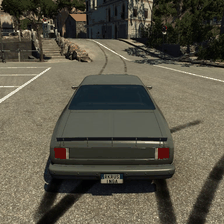
\includegraphics[width=0.5\columnwidth]{figures/v4_19_0.png} &
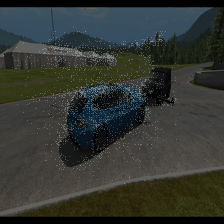
\includegraphics[width=0.5\columnwidth]{figures/v18_2_42.png}  \\
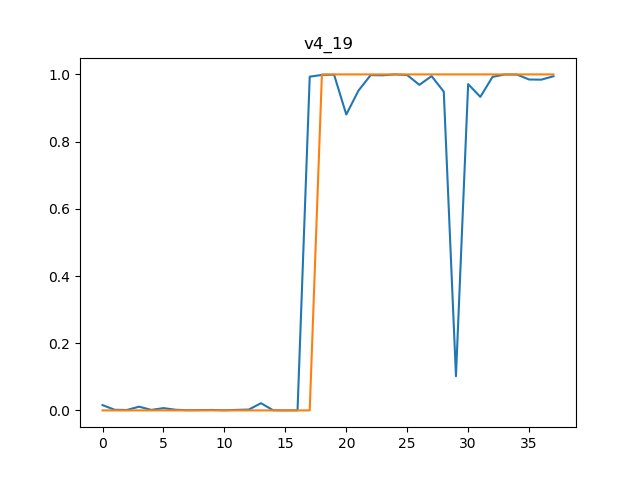
\includegraphics[width=0.5\columnwidth]{figures/v4_19_plot.png} &
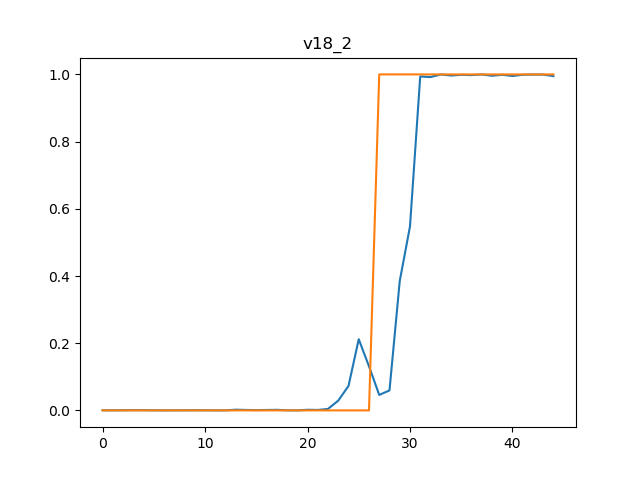
\includegraphics[width=0.5\columnwidth]{figures/v18_2_plot.png} 
\end{tabular}
\caption{Top left: a frame from one of the car videos. Top right: a frame from one of the crashes, overlayed by the most salient pixels. Bottom left: the crash prediction curve for the top left video. Bottom right: the crash prediction curve for the top right video.}
\end{figure}


%\begin{figure}
%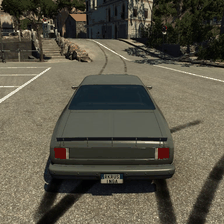
\includegraphics[width=\columnwidth, height=\columnwidth]{figures/v4_19_0.png}
%\end{figure}
%
%\begin{figure}
%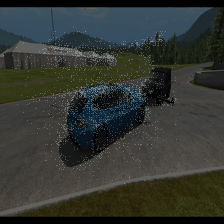
\includegraphics[width=\columnwidth, height=0.75\columnwidth]{figures/v18_2_42.png}
%\end{figure}
%
%\begin{figure}
%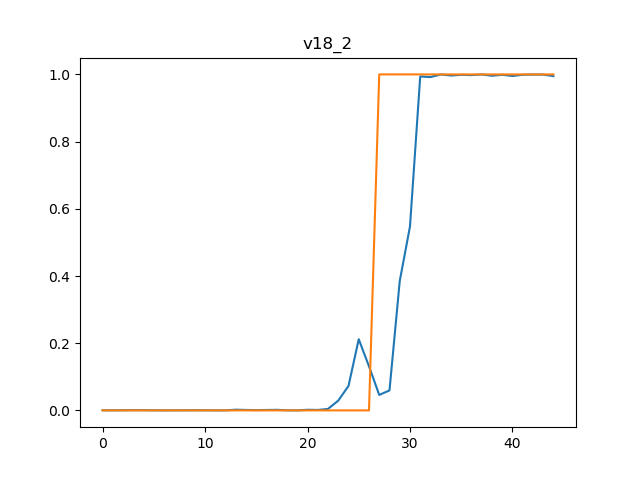
\includegraphics[width=\columnwidth, height=0.75\columnwidth]{figures/v18_2_plot.png}
%\end{figure}



%\section{Model and Results}
%
%
%
%\section{Conclusion}


% Outline of the rest:

% Brief introduction to causal thinking, and why most machine learning doesn't do it, and our method
% Judea Pearl's causality, potential outcomes, and related papers
% Modern papers attempting to incorporate deep learning and causality
% How reinforcement learning relates to causality
% Relation of gradients to causes

% Next section: Deep dive into formalism and metrics for measuring causality

% Next section: Our method

% Next section: Our dataset

% Next section: our results

% Next section: conclusion and future work












%\nocite{*}
\bibliographystyle{plain}
\bibliography{sources}

\end{document}
